\documentclass[12pt,a4paper]{article}

\usepackage[margin=2.5cm]{geometry}
\usepackage[utf8]{inputenc}
\usepackage[brazil]{babel}
\usepackage{lmodern}
\usepackage{fancyhdr}
\usepackage{tocloft}
\usepackage{amsmath}
\usepackage{graphicx}
\usepackage{booktabs}
\usepackage{array}
\usepackage{float}
\usepackage{hyperref}
\usepackage{lastpage}
\usepackage{subcaption}
\usepackage{multirow}

\newcommand{\diameter}{\phi}

\graphicspath{{../../../imagens_gerais/} {puxamento/}} 

\pagestyle{fancy}
\fancyhf{} 
\setlength{\headheight}{52pt}
\lhead{
  \includegraphics[height=1.2cm]{lafe_logo_ingles.jpg} \\
  \small
  Doc ID: PLT0073 \quad
  Doc tipo: Relatório de fabricação \quad
}
\rhead{
  \small \textbf{PLT0073 Suspended core em PETG esverdeado} \\
  Page \thepage\ of \pageref{LastPage}
}
\lfoot{\small \textcopyright\ 2026 LaFE. All rights reserved.}
\rfoot{\small Última data de revisão: 11/06/2026}

\begin{document}

\tableofcontents
\newpage

  Descrição da participação dos envolvidos na fabricação desta fibra:
  \begin{itemize}
    \item Ivan Prearo: Fabricação e puxamento
  \end{itemize}

  \section{Geometria e material}
  \label{sec:geometria}

  Comentários gerais sobre esta etapa:
  \begin{itemize}
    \item Pré-forma:
    \begin{itemize}
      \item Material: PETG esverdeado;
      \item Comprimento total: \(L_T = 90 mm\);
      \item Comprimento útil: \(L = 58 mm\); 
      \item Diâmetro externo: \(\diameter_e = 70 mm\)
      \item Geometria da secção transversal: \textit{Suspended-core};
      \item Diâmetro do núcleo: \(\diameter_n = 9.6 mm\);
      \item Espessura do cladding: \(L_c = 12 mm\);
      \item Largura dos \textit{struts}: \(L_s = 0.6 mm\);
      \item Número de \textit{struts}: \(N_s = 3\);
      \item Razões entre medidas iniciais na Tabela \ref{tab:puxamento1_razoes_das_dimensoes}
    \end{itemize}
    \item Objetivo: Fabricação de fibra suspended-core com \textit{struts} finos.
    \item O esquema da geometria da secção transversal e a foto da pré-forma são mostrados em Fig.~\ref{fig:puxamento1_geometria_preforma}.
  \end{itemize}

  \begin{table}[H]
  \centering
  \begin{tabular}{c|c|c}
    Dimensão & Medida [mm] & Razão com $\diameter_e$ \\
    \hline
    $\diameter_c$ & 70 & 1 \\
    $\diameter_n$ & 9.6 & 0.137 \\
    $L_s$ & 0.6 & 0.0086 \\
    $L_c$ & 12 & 0.171
  \end{tabular}
  \caption{Relações entre medidas relevantes da preforma}
  \label{tab:puxamento1_razoes_das_dimensoes}
  \end{table}

  \begin{figure}[H]
    \centering
    \begin{subfigure}{0.45\textwidth}
      \centering
      
\includegraphics[width=\linewidth]{images/Esquema_sec_transversal.png}
      \caption{Seção transversal.}
    \end{subfigure}
    \hfill
    \begin{subfigure}{0.45\textwidth}
      \centering
      
\includegraphics[width=\linewidth]{images/Preforma.jpeg}
      \caption{Foto.}
    \end{subfigure}
    \caption{Esquema do geometria da secção transversal e foto da pré-forma.}
    \label{fig:puxamento1_geometria_preforma}
  \end{figure}


  \section{Puxamento}
  \label{sec:puxamento}

  Por erros de informação das distâncias entre furos da tampa, não foi possível inserir ambos os pinos nas tampas.
  Portanto, a preforma foi puxada com um pino em cada extremidade.

  \subsection{Primeiro puxamento}
  \label{subsec:puxamento1}

    A rampa de secagem/recozimento é apresentada na Tab.~\ref{tab:puxamento1_fase1_etapa2_rampa}.
    Nota-se que após o primero escoamento, iniciou-se uma tentativa de puxamento que falhou pela preforma não estar na temperatura correta.
    Essa primeira tentativa causou uma deformação significativa na preforma, principalmente na direção sem pino como mostrado na Figura \ref{fig:puxamento_falho}, mas a preforma foi realinhada e mantida a 120$^\circ$C, testando se escoava ou não de 10 em 10 minutos.
    Após mais 40 minutos nessa temperatura, notou-se escoamento e uma nova tentativa de puxamento foi realizada.

    \begin{table}[H]
    \centering
    \begin{tabular}{ccc}   
      \toprule 
      \textbf{Fase} & \textbf{[°C]} & \textbf{Tempo [min]} \\ 
      \midrule
      \multirow{1}{*}{Secagem} & 60 & 60 \\
      \midrule
      \multirow{1}{*}{Amolecimento} & 80 & 60 \\
      \midrule
      \multirow{3}{*}{Escoamento} & 100 & 30 \\
                               & 110 & 15 \\ 
                               & 120 & 5 \\ 
      \midrule
      \multirow{1}{*}{Tentativa de puxamento} & 120 & 10 \\ 
      \midrule
      \multirow{1}{*}{Escoamento 2} & 120 & 40 \\ 
      \midrule
      \multirow{1}{*}{Puxamento} & 120 & \(\infty\) \\
      \bottomrule
    \end{tabular}
    \caption{Rampa de temperatura no forno da torre antes e durante o puxamento.}
    \label{tab:puxamento1_fase1_etapa2_rampa}
  \end{table}

  \begin{figure}[H]
    \centering
    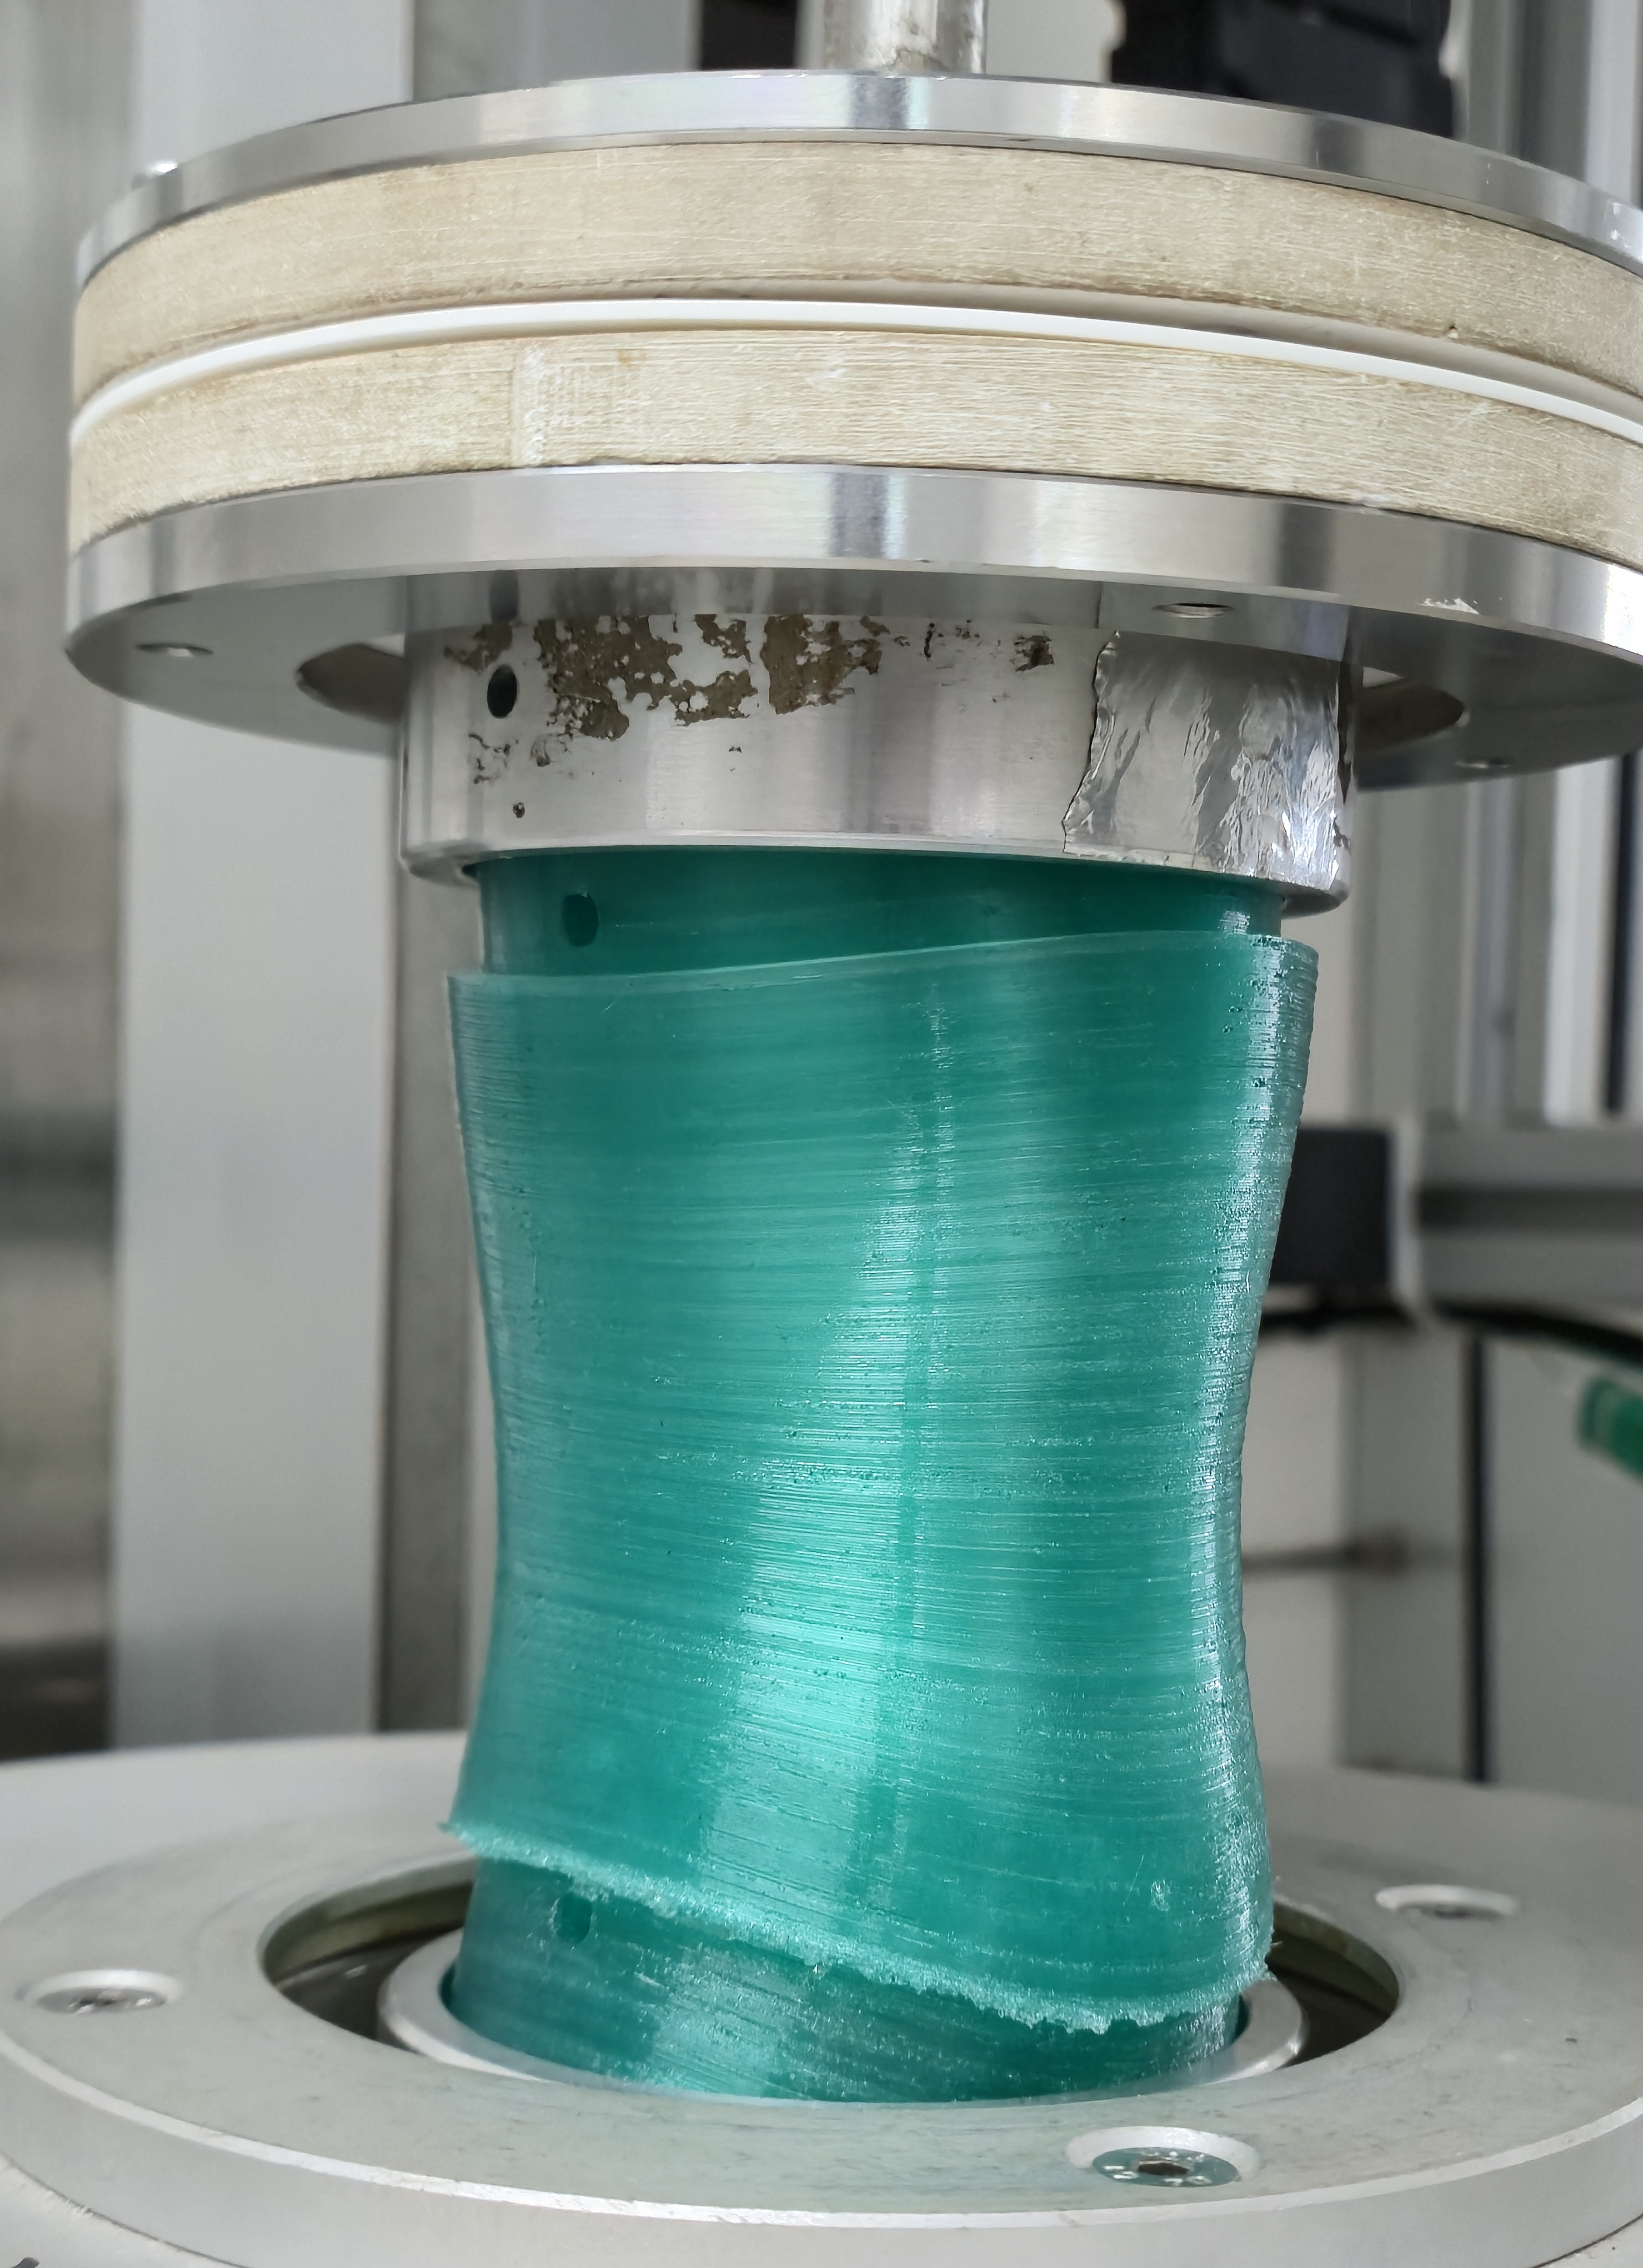
\includegraphics[width=0.5\linewidth]{images/Falha_puxamento.jpg}
    \caption{Puxamento falho por rampa de temperatura curta demais.}
    \label{fig:puxamento_falho}
  \end{figure}

  Após a rampa total mostrada na Tabela \ref{tab:puxamento1_fase1_etapa2_rampa}, o puxamento ocorreu normalmente e o resultado foi um \textit{cane} de 56 cm de comprimento homogêneo com diâmetro de 9 a 11 cm (Fig. \ref{fig:cane_total}).

  \begin{figure}[H]
    \centering
    
    \begin{subfigure}{0.9\linewidth}
      \centering
      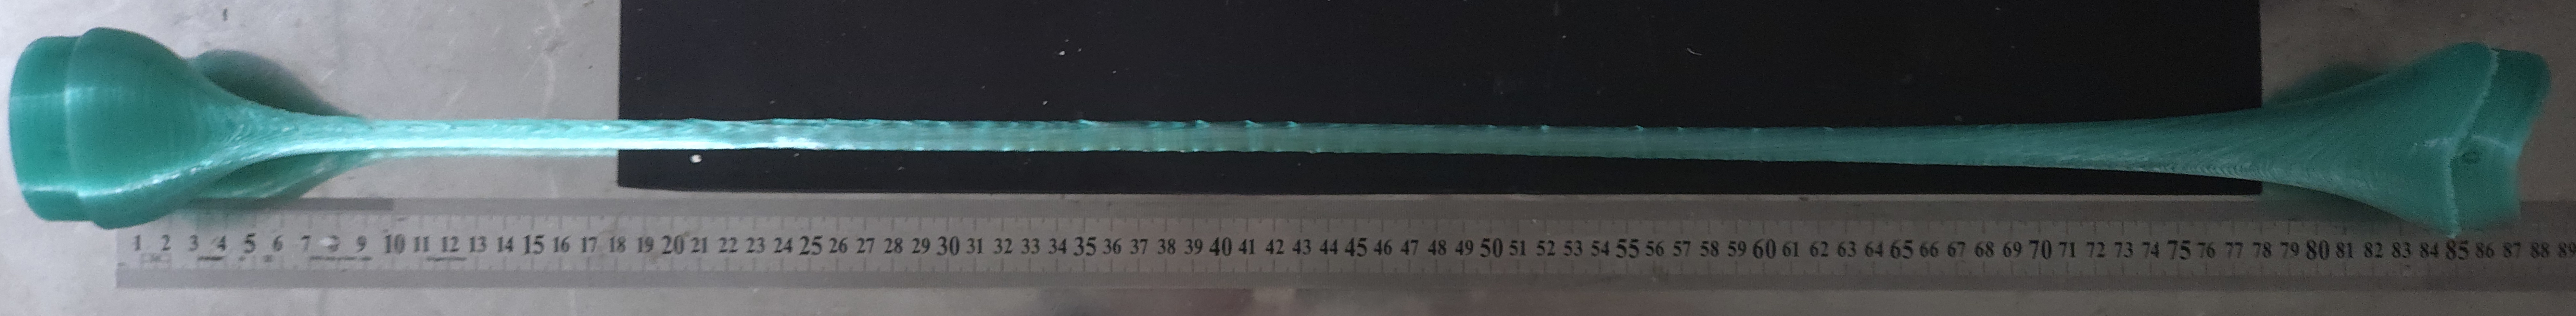
\includegraphics[width=\linewidth]{images/Cane_produzido.jpg}
      \caption{\textit{Cane} total.}
      \label{fig:cane_total}
    \end{subfigure}
    
    \begin{subfigure}{0.9\linewidth}
      \centering
      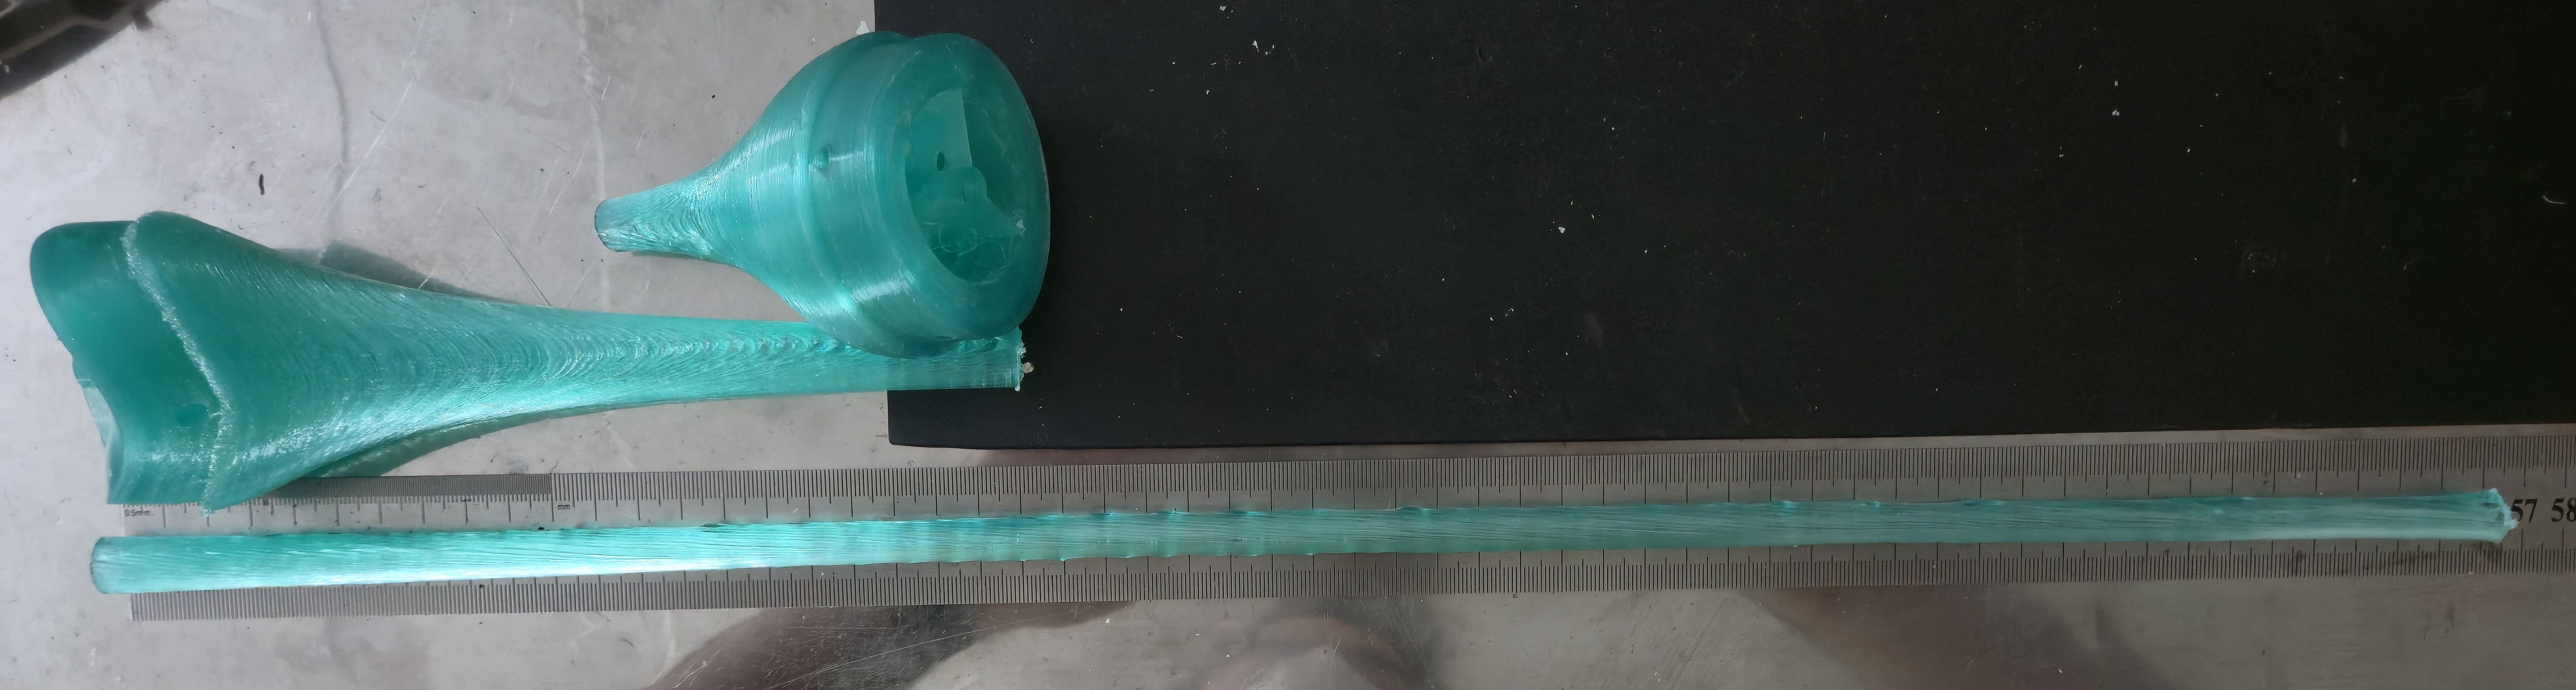
\includegraphics[width=\linewidth]{images/Cane_cortado_medida.jpg}
      \caption{Medida do \textit{cane} homogêneo.}
      \label{fig:cane_medida}
    \end{subfigure}

    \begin{subfigure}{0.9\linewidth}
      \centering
      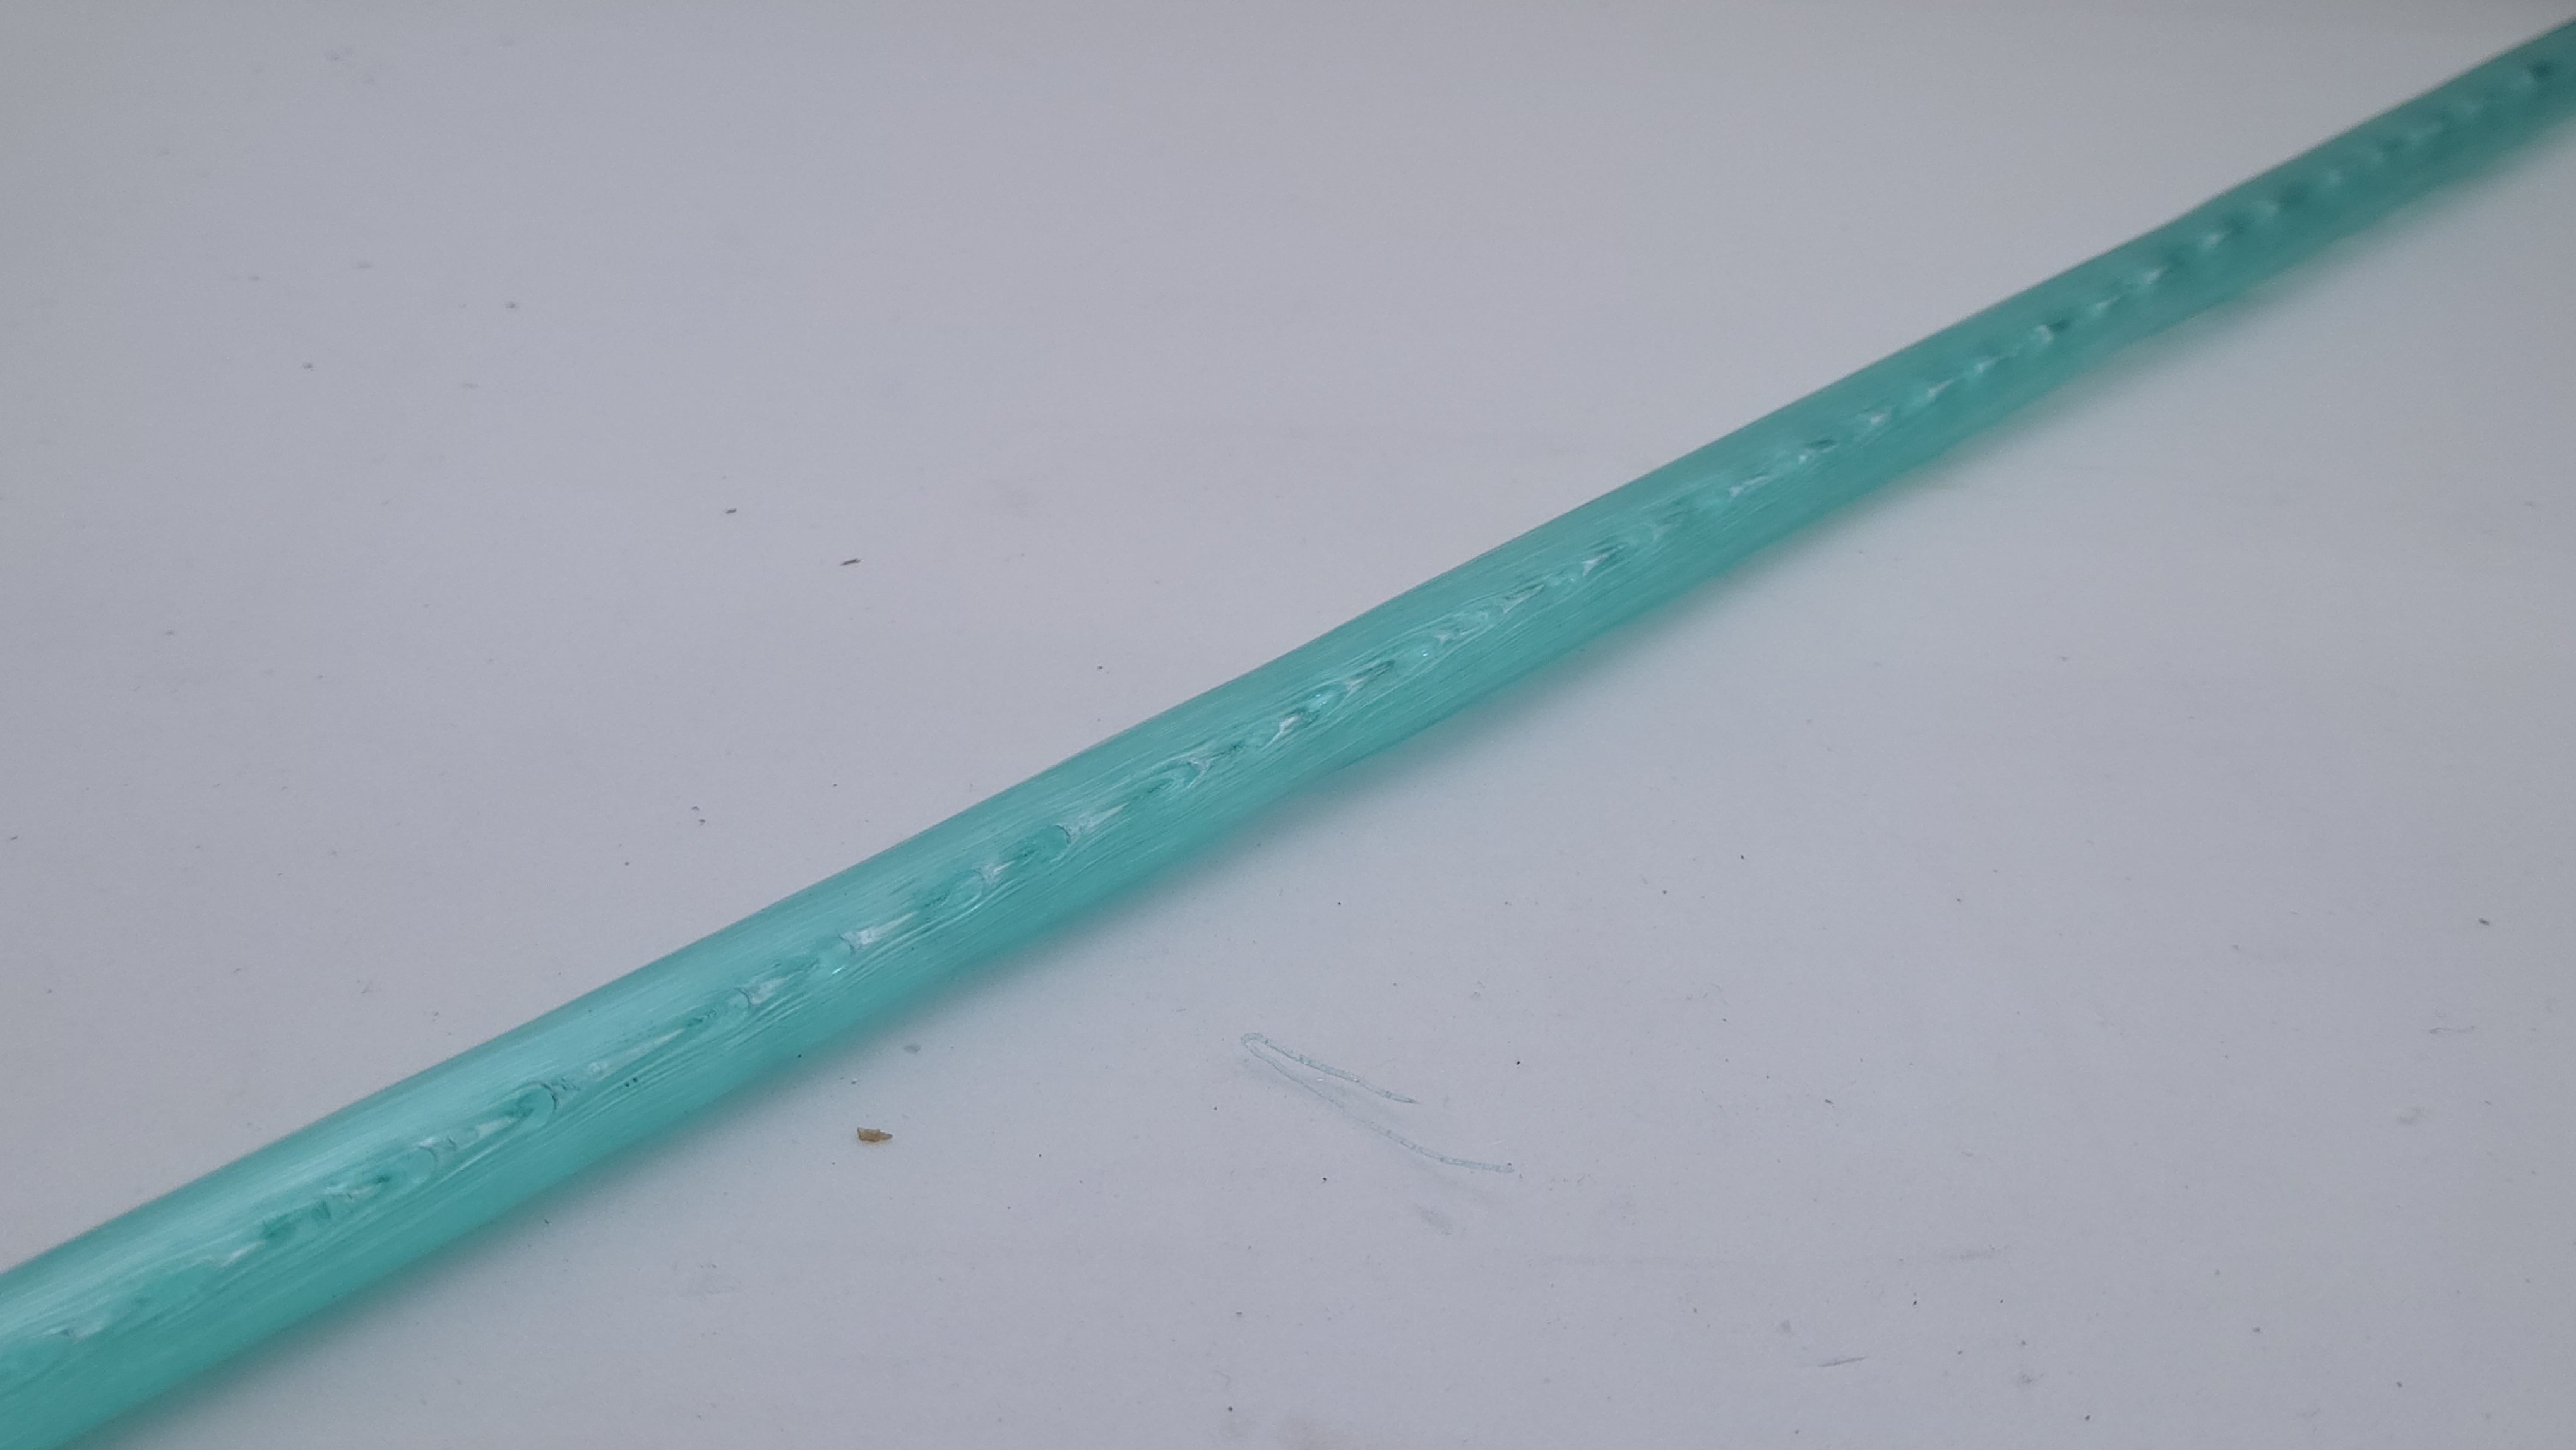
\includegraphics[width=\linewidth]{images/Cane_final.jpg}
      \caption{Foto aproximada.}
      \label{fig:cane_foto}
    \end{subfigure}

    \caption{\textit{Cane} produzido e sua respectiva medida de comprimento total.}
    \label{fig:cane_puxado}

  \end{figure}

  Durante o puxamento, por conta das deformações ocorridas antes do segundo período de escoamento, uma das struts se desfez (Fig. \ref{fig:sec_transversal_cane}).
  Além disso, é notável que os outros \textit{struts} ficaram demasiadamente finos e, em alguns locais, quebrados.
  Para amostras futuras, é recomendada a impressão de struts maiores.

  \begin{figure}[H]
    \centering
    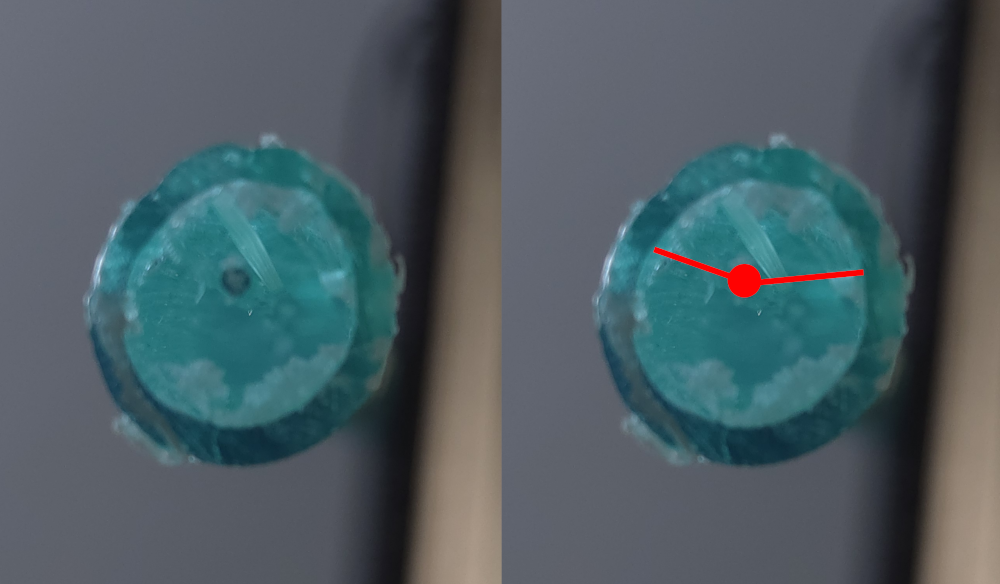
\includegraphics[width=0.7\linewidth]{images/Cane_anotado.png}
    \caption{Seção transversal produzida. Em vermelho está anotada a estrutura restante no \textit{cane}.}
    \label{fig:sec_transversal_cane}
  \end{figure}

  \subsection{Armazenamento}
  \label{subsubsec:puxamento1_fase1_etapa3}

  \textit{Descrição desta etapa:} armazenamento da amostra

  Comentários gerais sobre esta etapa:
  \begin{itemize}
    \item Amostra armazenada a 60$^\circ$C, sem apresentar sinais de deterioração durante os 8 dias que foi mantida na estufa.
  \end{itemize}

  
  \subsection{Segundo puxamento}
  \label{subsec:puxamento2}

  \subsubsection{Primeira tentativa}
  \label{subsubsec:puxamento2_tentativa1}

  Comentários gerais sobre esta tentativa:
  \begin{itemize}
    \item Data de puxamento: 11/06/2026.
    \item A rampa de puxamento é mostrada na Tabela \ref{tab:puxamento1_fase2_etapa1_rampa}.
    \item Resultou em falha.
  \end{itemize}

  O \textit{cane} produzido durante o primeiro puxamento teve furos feitos utilizando uma microrretífica para a inserção da tampa do extensor.
  Após os 10 minutos de escoamento a 120$^\circ$C, abriu-se o clamp do tractor a fim de testar a velocidade de escoamento pelo peso do extensor.
  Neste momento, o escoamento era rápido demais e, após 5 minutos de puxamento foi tomada a decisão de diminuir a temperatura ligeiramente, para 115$^\circ$C.
  No entanto, após a transição do extensor para a fibra no tractor, notou-se uma força contrária forte o suficiente para impedir o puxamento apenas do tractor.
  Após alguns minutos disso, a fibra sendo puxada com cerca de 1mm de diâmetro se rompeu (Figura \ref{fig:primeira_tentativa_res}).
  Há a teoria de que isso ocorreu pelo resfriamento da seção que estava sendo puxada, enquanto a tensão era mantida.
  Esse resfriamento foi primariamente atribuído à diminuição da temperatura durante o puxamento, mas há a possibilidade de que a amostra não estava sendo aquecida o suficiente durante a passagem pelo forno, diminuindo a temperatura real da amostra.

  \begin{table}[H]
    \centering
    \begin{tabular}{ccc}   
      \toprule 
      \textbf{Fase} & \textbf{[°C]} & \textbf{Tempo [min]} \\ 
      \midrule
      \multirow{1}{*}{Secagem} & 60 & 60 \\
      \midrule
      \multirow{1}{*}{Amolecimento} & 80 & 60 \\
      \midrule
      \multirow{3}{*}{Escoamento} & 100 & 30 \\
                                  & 110 & 15 \\
                                  & 120 & 10 \\
      \midrule
      \multirow{2}{*}{Puxamento} & 120 & 5 \\
                                 & 115 & $\infty$ \\
      \bottomrule
    \end{tabular}
    \caption{Rampa de temperatura no forno da torre antes do puxamento.}
    \label{tab:puxamento1_fase2_etapa1_rampa}
  \end{table}

  \begin{figure}[H]
    \centering
    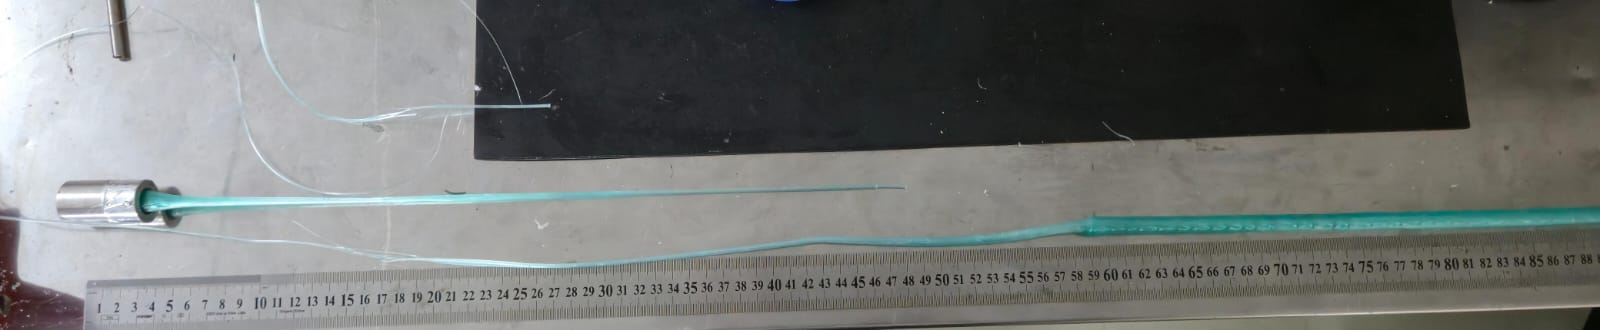
\includegraphics[width=\linewidth]{images/Resultado_primeira_tentativa.jpeg}
    \caption{Foto do resultado final da primeira tentativa.}
    \label{fig:primeira_tentativa_res}

  \end{figure}

  De qualquer maneira, a amostra foi mantida no forno parada a fim de recomeçar o puxamento, mas após diversos aumentos de temperatura ao longo de 1 hora, o teste de escoamento não demonstrava que a preforma havia chegado no ponto de puxamento.
  Isso indica que houve acúmulo de tensão interna no material, então a amostra foi cortada até a região de diâmetro constante e colocada novamente na estufa a 60$^\circ$C para puxamento posterior.
  O comprimento total de 56cm foi diminuído para 44cm durante este puxamento, o que ainda corresponde a uma amostra significativamente maior do que o atingido pela impressão direta em 15mm.

  \subsubsection{Segunda tentativa}
  \label{subsubsec:puxamento2_tentativa2}

  % \section{Resultados}
  % \label{sec:puxamento_resultados}

  % Comentários gerais dos resultados:
  % \begin{itemize}
  %   \item A foto do primeiro estágio produzido é mostrada em Fig.~\ref{fig:puxamento1_resultados_estagio1}.
  %   \item O gráfico do perfil the diâmetro do primeiro estágio é mostrado em Fig.~\ref{fig:puxamento1_resultados_perfil}.
  % \end{itemize}

  % \begin{figure}[H]
  %   \centering
  %     \begin{subfigure}{0.45\textwidth}
  %     \centering
  %     \includegraphics[scale=0.5]{}
  %     \caption{Foto do primeiro estágio.}
  %     \label{fig:puxamento1_fase2_resultados_estagio1}
  %   \end{subfigure}
  %   \hfill
  %   \begin{subfigure}{0.45\textwidth}
  %     \centering
  %     \includegraphics[scale=0.5]{}
  %     \caption{Perfil do diâmetro do primeiro estágio.}
  %     \label{fig:puxamento1_resultados_perfil}
  %   \end{subfigure}
  %   \caption{}
  % \end{figure}
  
  % \section*{Puxamento 2}
  % \label{sec:puxamento2}

  % Data de puxamento: dd/mm/aaaa.

  % A rampa de temperatura do segundo puxamento é mostrada na Tab.~\ref{tab:puxamento2_fase2_rampa}.

  % \begin{table}[H]
  %   \centering
  %     \begin{tabular}{|c|c|} \hline
  %       \textbf{ [°C]} & \textbf{Tempo [min]} \\ \hline
  %       120 & 30 \\
  %       150 & 30 \\
  %       170 & 30 \\ 
  %       190 & 5 \\ 
  %       200 & 2 \\ \hline
  %     \end{tabular}
  %   \caption{Rampa de temperatura no forno da torre para o segundo puxamento.}
  %   \label{tab:puxamento2_fase2_rampa}
  % \end{table}

  % \subsection*{Resultados}
  % \label{subsec:puxamento2_resultados}

  % Comentários gerais dos resultados:
  % \begin{itemize}
  %   \item A foto das fibras catalogadas é mostrada na Fig.~ \ref{fig:puxamento2_fase2_resultados_catalogacao}.
  %   \item As micrografias das bandas ? são mostradas na Fig. ~\ref{fig:puxamento2_fase2_resultados_micrografias}.
  %   \item Os parâmetros de puxamento de cada banda estão organizados na Tab.~\ref{tab:puxamento2_fase2_resultados_parametros}.
  %   \item Os principais gráficos de fabricação gerados pela torre de polímero com todas as bandas juntas são mostrados em Fig.~\ref{fig:puxamento2_fase2_resultados_graficosjuntos}. 
  % \end{itemize}

  % \begin{figure}[H]
  %   \centering
  %   \includegraphics[scale=0.2]{}
  %   \caption{Fibras catalogadas.}
  %   \label{fig:puxamento2_fase2_resultados_catalogacao}
  % \end{figure}

  % \begin{figure}[H]
  %   \centering
  %   \begin{subfigure}{0.45\textwidth}
  %     \centering
  %     \includegraphics[scale=0.1]{}
  %     \caption{Banda ?.}
  %   \end{subfigure}
  %   \begin{subfigure}{0.45\textwidth}
  %     \centering
  %     \includegraphics[scale=0.1]{}
  %     \caption{Banda ?.}
  %   \end{subfigure}
  %   \caption{Micrografias das bandas ?.}
  %   \label{fig:puxamento2_fase2_resultados_micrografias}
  % \end{figure}

  % \begin{table}[H]
  %   \centering
  %     \begin{tabular}{|c|c|c|c|c|c|c|} \hline
  %       \textbf{Band} & $\mathbf{D_{ext} [\mu m]}$ & \textbf{T [°C]} & \textbf{P [mbar]} & $\mathbf{\tau [g]}$ & $\mathbf{\epsilon_{norm}}$ & $\mathbf{\epsilon_{geo}}$ \\ \hline
  %       ? & $ \pm  $ & $  \pm  $ & $  \pm  $ & $ \pm  $ & $ \pm  $ & $ \pm  $ \\
  %       ? & $ \pm $ & $ \pm $ & $ \pm $ & $ \pm $ & $ \pm  $ & $ \pm  $ \\ \hline
  %     \end{tabular}
  %   \caption{Parâmetros de puxamentos para bandas ?.}
  %   \label{tab:puxamento2_fase2_resultados_parametros}
  % \end{table}

  % \begin{figure}[H]
  %   \centering
  %   \begin{subfigure}{0.45\textwidth}
  %     \centering
  %     \includegraphics[scale=0.5]{}
  %     \caption{Pressão.}
  %   \end{subfigure}
  %   \hfill
  %   \begin{subfigure}{0.45\textwidth}
  %     \centering
  %     \includegraphics[scale=0.5]{}
  %     \caption{Tensão.}
  %   \end{subfigure}
  %   \begin{subfigure}{0.45\textwidth}
  %     \centering
  %     \includegraphics[scale=0.5]{}
  %     \caption{Diâmetro médio.}
  %   \end{subfigure}
  %   \caption{Principais gráficos dos parâmetros de puxamentos com todas bandas juntas.}
  %   \label{fig:puxamento2_fase2_resultados_graficosjuntos}
  % \end{figure}

\end{document}